\section{Objects' representation and processing for best grasp computation}
After recognizing the objects which are present into the scene and having a
good pose estimation, the robot used for objects' picking must compute the best path
in which to travel in order to correctly grasp it. In this project, this task
is accomplished by simulating a set of predefined poses over each object before
gripping. As the goal of the project is grasping a \emph{set} of objects, a
good grasping strategy must be implemented too; this strategy is described in
detail in sec. \ref{sec:order-list}. However, this means that, independently from the
chosen global strategy, grasping pose computation has to assign to each
possible set of movements (which we will refer to as a \emph{grasp} from now on)
a \emph{score} representing the difficulty of picking
for that particular grasp. The chosen algorithm assigns to each grasp a
probabilistic score, based on the intersection volume between an emulated
gripper and the scene, from which the object to grasp has been removed.

In this section, first it is described the score concept (sec.
\ref{sec:grasp_score}), then the chosen way of modelling the gripper (and robot) and
the scene (sec. \ref{sec:shapes}). Finally, a flexible way to compute the score for a set of possible
grasps is presented, together with details for particular cases (sec.
\ref{sec:grasp_computing}).

\subsection{Probabilistic grasping score} \label{sec:grasp_score}
For the implementation of any high-level grasping strategy for multiple
objects, i.e. for the program to be able to correctly choose which object to
pick first at each time instant, a score has been assigned to each possible
grasp and for each possible object. For each pickable object, only the best
grasping poses are kept.

In order to well define the score (i.e. difficulty) of a grasp, which we will
indicate as $d$, a few
considerations have been done:
\begin{itemize}
  \item{First, an easy to do grasp with no obstacles
      into its path shall have score $d=0$. It shall, in fact, be  the preferred
    object for the high-level strategy to pick first;}
  \item{on the other hand, a grasp which puts the
      gripper at risk of hitting the borders of the object's container -- being them
      the edges of a bin or the floor -- shall have score $d=+\infty$. Trying to pick the
      object with this grasp could cause physical damage to the robot, the floor or
    even humans, thus the high-level strategy should discard it completely;}
  \item{if a grasp puts the gripper in contact with other objects of a scene, its
      difficulty can be evaluated by virtually assuming these objects will stay still and
      computing the intersection volume $V_{\text{int}}$ between them and the
      gripper for each of them;}
    \item{If the intersection volume $V_{\text{int}}$ is small enough to be
        under a certain threashold $V_{\text{easy}}$, the score could be assigned low enough for the
      grasp to be considered valid. In this way, if the gripper brushes the object
      without entering it completely, the grasp can be done, which in real situations
      will result in the gripper slightly moving apart the touched object without
    damaging it; }
  \item{the intersection volume, especially is considered to grow linearly, is not
      enough for evaluating the score: first, the score must grow consistently if the
      object is not touched only by the border but by a consistent part of the
      gripper, and finally saturate to $d=+\infty$ if the intersection volume
      reaches an acceptability threshold $V_{\text{max}}$. Also, as touching an object will result in moving it, grasp score
      should keep into account the actual difficulty of moving the intersected
      object. For example, bouncing with a closed, rigid box would probably not damage it
      also if the gripper enters it by a visible amount, while bouncing with an
      open book would almost for sure damage its pages. Thus, a \emph{movement
    coefficient} shall be assigned to each of the objects into the scene.}
\end{itemize}


With these considerations in mind, a suitable, global score function $s(V_{\text{int}})$
can be found. The score function must obey certain properties which can be
extracted from the above:

\begin{enumerate}
  \item{The function must be monotonic and always positive;}
  \item{it must be linear when x is low enough, in order to evaluate
    lightly touches adequately;}
  \item{it must be continue in the whole domain: this does not come
      from the previous properties, but is needed in order to compute it without
    the need of caring about floating point's approximations;}
  \item{it must have a parameter $\alpha>0$ defining how much
    intersection volume globally affects hardness of grasp;}
  \item{it must have another parameter $K\geq1$ defining how much the hardness is
    increased rapidly after reaching the brushing threshold $V_{easy}$;}
  \item{when the intersection volume is greater than the brushing threshold, the
      function
    must never grow less quickly than when the volume is in the brushing
    region, i.e. $\text{max}\left( \left\{ \frac{ds(x)}{dx} | 0 \leq
    x \leq V_{\text{easy}} \right\} \right) \leq \text{min}\left( \left\{
  \frac{ds(x)}{dx} | x > V_{\text{easy}}\right\} \right)$.}
\end{enumerate}

The chosen function, which satisfies all of the above properties, is

\begin{equation} \label{eqn:score-function}
  s(V_{\text{int}})=\left\{
    \begin{array}{lcr}
      \frac{\alpha}{V_{\text{easy}}} V_{\text{int}} & \text{when} & 0 \leq V_{\text{int}} \leq V_{\text{easy}}, \\
      \alpha
      \left[1-K\left(1+\frac{V_{\text{max}}-V_{\text{easy}}}{V_{\text{int}}-V_{\text{max}}}\right)\right]
      & \text{when} &  V_{\text{easy}} < V_{\text{int}} < V_{\text{max}}, \\
      +\infty & \text{when} & V_{\text{int}} \geq V_{\text{max}}.
    \end{array}
  \right.
\end{equation}

It is shown in appendix \ref{sec:demonstrate-score} that $s(V_{int})$ satisfies all
of the above properties for any $K\geq \frac{V_{\text{max}}-V_{\text{easy}}}{V_{\text{easy}}}$, and is thus suitable as a score
function. Some examples of this function varying the two parameters $\alpha$ and
$K$ are shown in fig. \ref{fig:score_function}.

\begin{figure}[htbp]
  \centering
  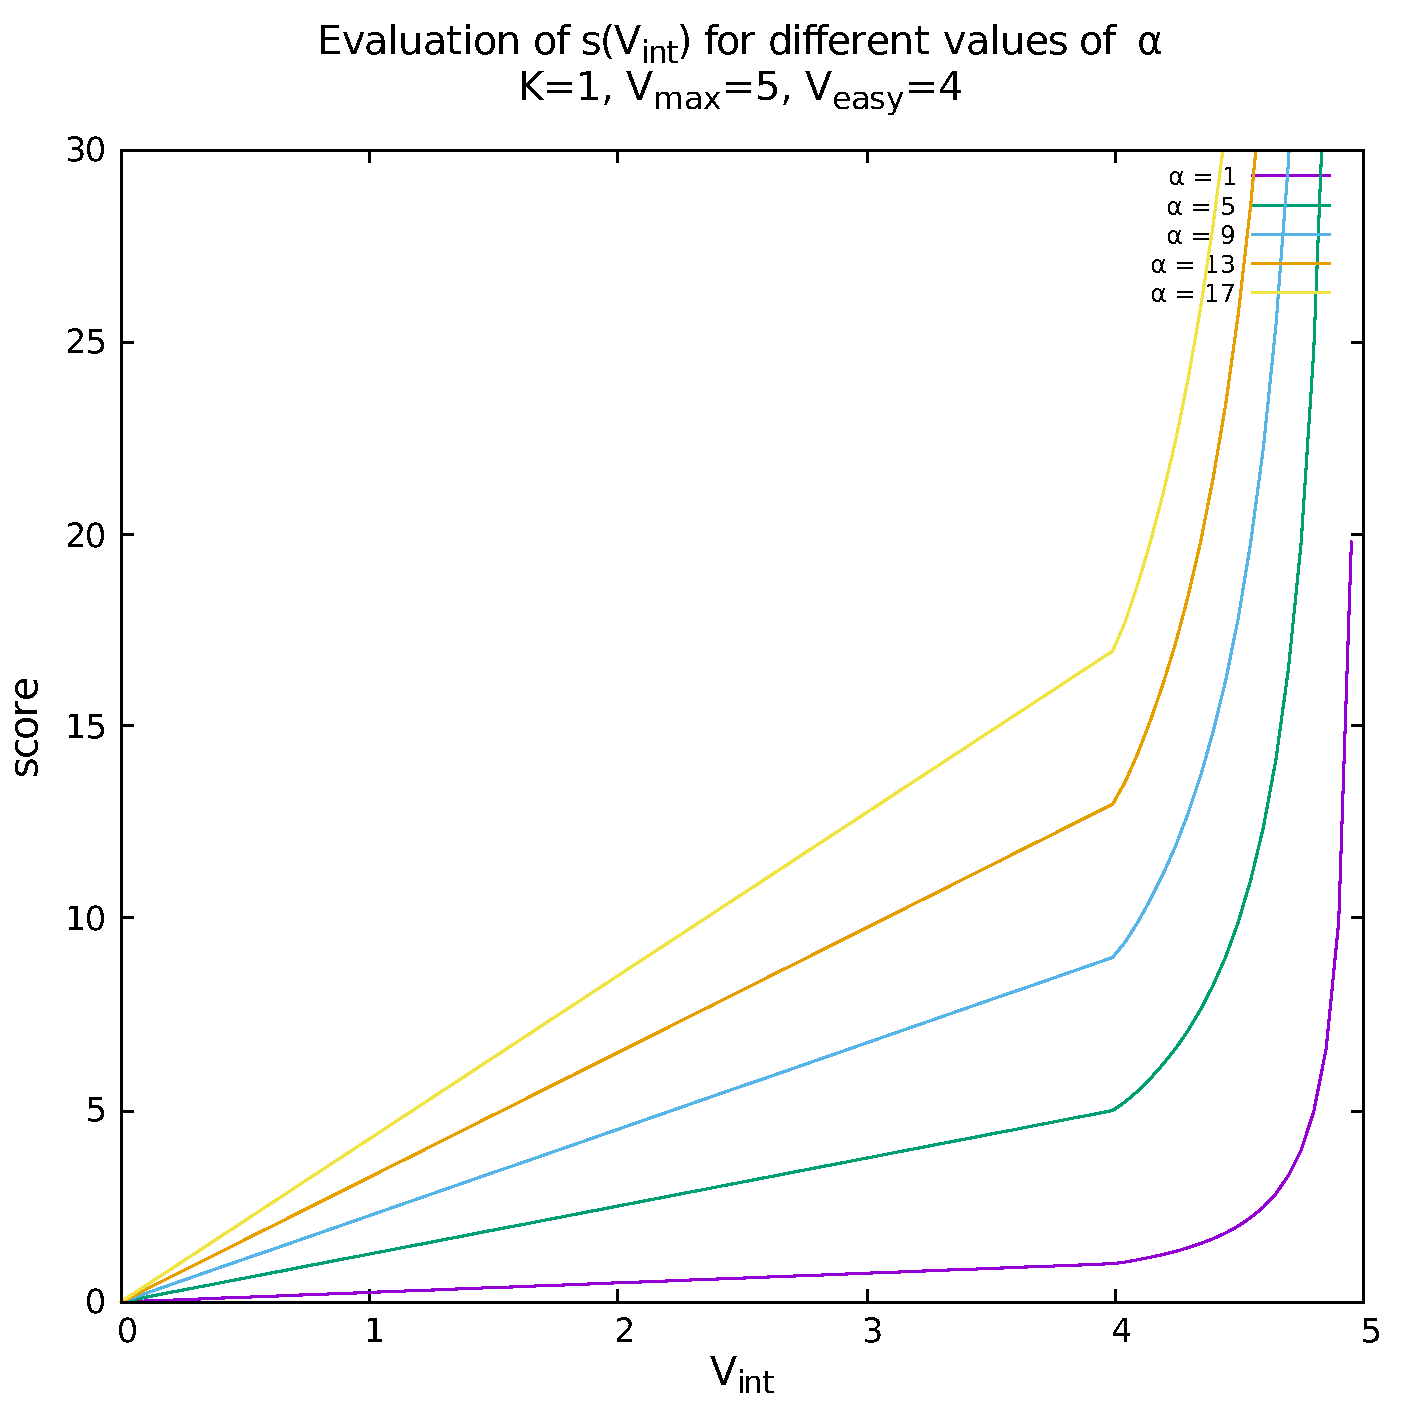
\includegraphics[height=3in]{./Graphics/score_alpha}
  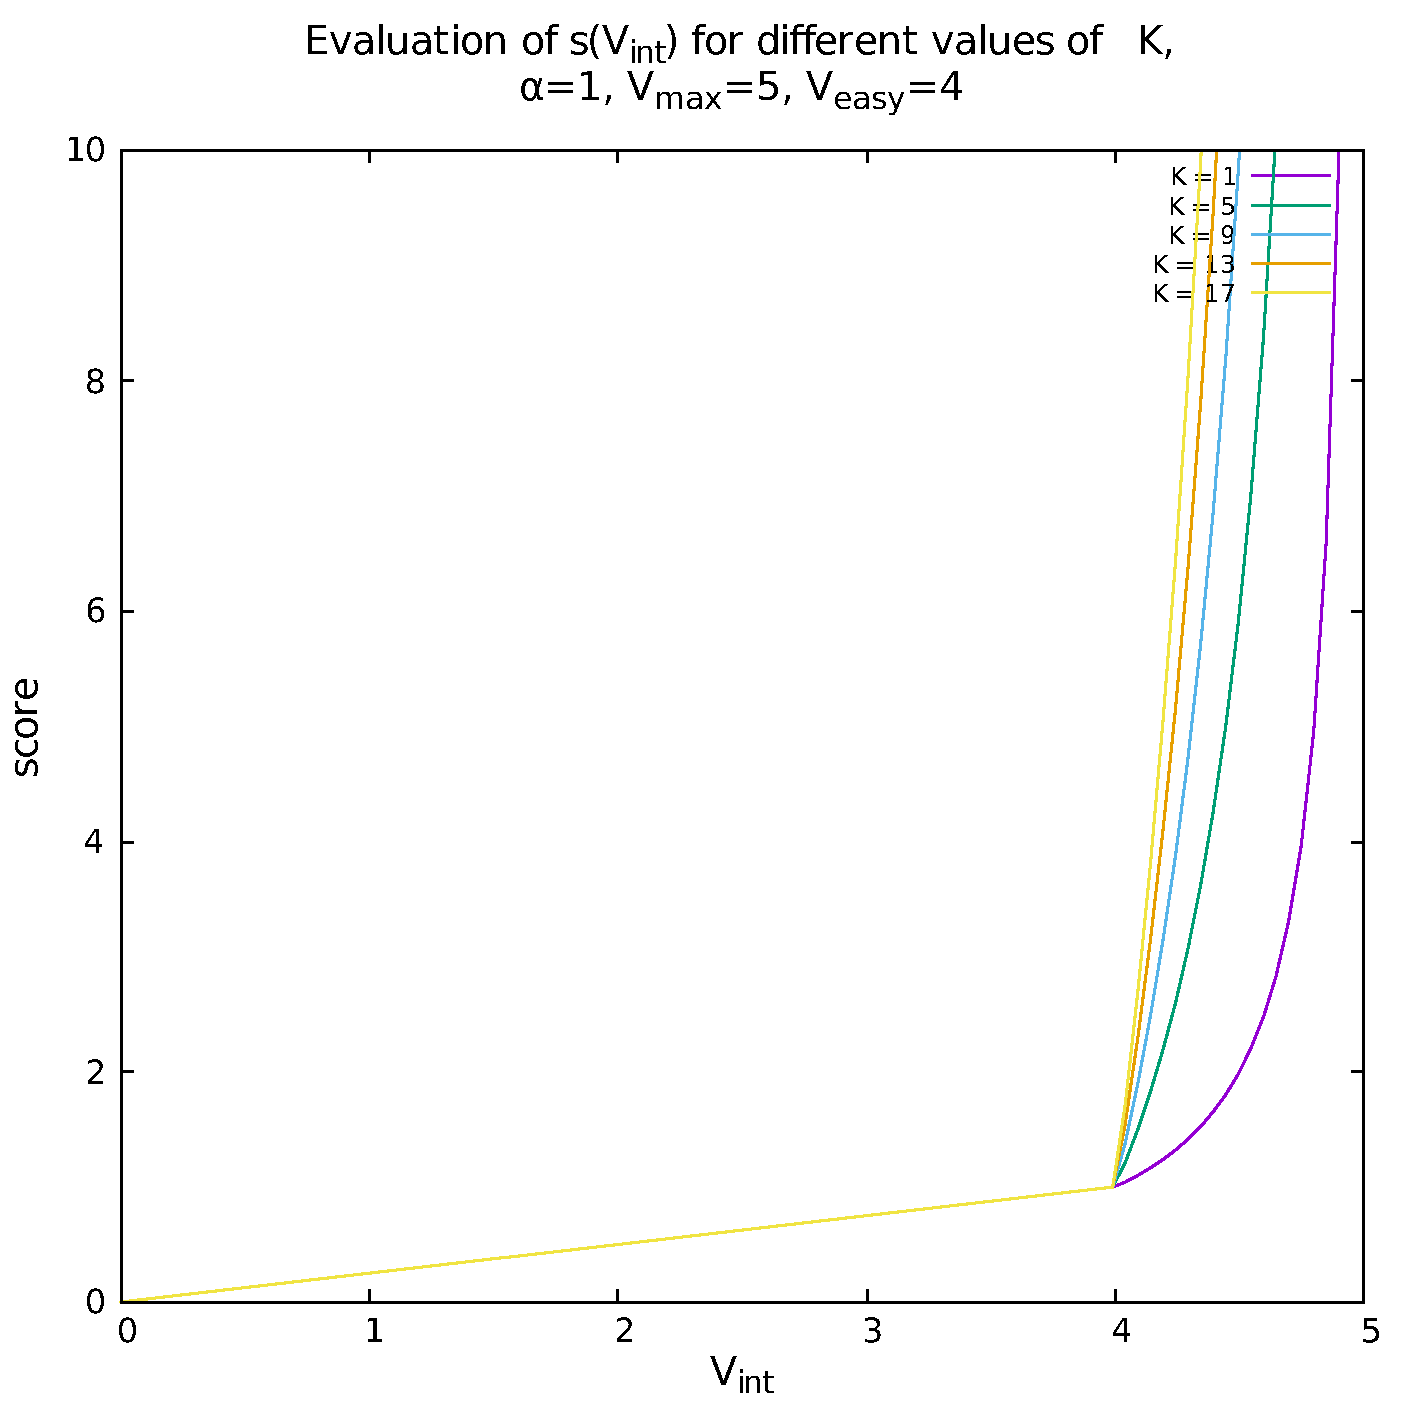
\includegraphics[height=3in]{./Graphics/score_k}
  \caption{Resulting score function for different values of $\alpha$ (top) and
  $K$ (bottom) \label{fig:score_function}}
\end{figure}

\subsection{Object representation as elementary shapes} \label{sec:shapes}
A good representation of objects is essential in order to compute efficiently
their intersection. In this project, objects have been represented by means of a
uniform data structure breaking down complex meshes to the union of simpler
shape, as done with the \emph{Constructive Solid Geometry (\emph{CSG})} tools of
most mainstream CAD applications. Each object is represented, for the purpose of
grasp computation, by means of simpler, basic shapes, associated to their pose
relative to the object's reference system. These will be called
\emph{primitives}. A tree structure can also be created
by considering compound objects created in this manner to be a shape type on
their own, thus allowing recursive object building. This is similar to what the
\emph{assembly} and \emph{group} tools of common CAD applications do, as well
as what the library used for mesh representation (Assimp) does for
multiple-nodes meshes. This approach has a serie of advantages:
\begin{itemize}
  \item{Every object shares a common data structure. This makes it easier for
      the intersection algorithm to be as general as possible with little to no
    effort;}
  \item{the tree representation of the object makes it easy to save single or
      multiple objects to file and to create objects' configuration by-hand,
      which is useful both for debugging and for execution purposes (for
      example, the database of objects, together with their shapes, can be made
    distributed with no effort and version control tools can be useful);}
  \item{using an approach similar to what is supported by CAD
      applications results in the possibility of scripting the latter in order
      to automatically produce an exact representation of the object starting
      from a CAD model, which could be the same used for training in sec.
    \ref{sec:cad-mesh};}
  \item{the approach is very flexible because of the relative independency
      between the object's model and the rest of the algorithms: new use-case of
      the algorithm (e.g. for moving or nonrigid objects) could leave this part intact, and
      only work by modifying the informations about the position of the whole,
    or part of, the object.}
  \item{new, complex shapes which have to be implemented in future can be added
      to the primitive shapes as an extension, without the need of rebuilding
      the whole objects' database. This is the main advantage of using an
      object-oriented approach based on polimorphism for the implementation of this
    part.}
\end{itemize}

For this project, four main shape types have been implemented, and with these
the whole set of objects kept in consideration have been succesfully
represented.

Each primitive is represented by its shape type and a set of dimensions, which
is checked at runtime to be coherent to the associated shape. To the shape is
associated a pose information, represented as an affine transformation as in the
rest of the project. To each shape type functions have been implemented to
recognize whether a it intersects with, or contains, a point, an edge, a line, or
another shape. When computing intersections, these are efficiently used as
special cases to recognize whether an intersection exists or not before
eventually running the computationally expensive intersection's volume
algorithm.

\paragraph{A \emph{cuboid}} is a shape representing a parallelepiped. It is represented by
three dimensions: its width $W$, its height $H$, and its depth $D$; its origin is fixed in one
of its corners, and its reference system's axis are on its edges' directions:
width extends over the $X$ axis, height extends over the $Y$ axis, and depth
extends over the $Z$ axis.

A point $P$ (in normalized homogeneous coordinates, i.e. with $w=1$  can be checked for belonging a cuboid $C$ of dimensions $(W,H,D)$ and
pose $A$ by first representing it into
the cuboid's coordinate system, and then checking its coordinates to be into the
cubes'dimensions:

\begin{equation}
P \in C \Leftrightarrow \begin{pmatrix}0\\0\\0\\1\end{pmatrix} \leq A^{-1}P \leq
\begin{pmatrix}W\\H\\D\\1\end{pmatrix}
\end{equation}
  
A line segment $L$ intersects the same cuboid if, by projecting it on one axis at a time,
all the three projections belong to the projection of the cube:

\begin{equation}
  L \in C \Leftrightarrow \left(L_x \in C_x\right) \wedge
  \left(L_y \in C_y\right) \wedge \left(L_z
    \in C_z\right)
\end{equation}

\paragraph{A \emph{sphere}} is a shape representing a sphere of fixed radius,
which is the only one of its dimensions. The reference system of the sphere, 
which its transformation refers to, is fixed into the sphere's center. Having
central simmetry, the rotation part of the sphere's transformation will actually
be ignored.

A point $P$ belongs to a sphere $S$ of radius $R$ if, after moving it into the
sphere's reference system, its distance from the origin is less then the radius:

\begin{equation}
  P \in S \Leftrightarrow \left(A^{-1}P\right)_{x,y,z}^2 < R^2
\end{equation}

Also, a line $L$ belongs to the same sphere if its distance from the origin is less
than $R$.

\paragraph{A \emph{cylinder}} is a shape representing a rect, circular cylinder.
Its two dimensional values represent the base's radius and the height of the
cylinder. Its coordinate system is fixed at the center of the circle, at the
base of the cylinder, with the
Z axis pointing upwards on the length direction.

A point $P$ belongs to a cylinder $C$ of radius $R$ and height $H$ if, after
moving it to the cylinder's reference system, its projection on the XY plane
belongs the base circle and its Z coordinate is lower than the cylinder's
height:

\begin{equation}
  P \in C \Leftrightarrow \left(A^{-1}P\right)_{x,y}^2 < R \wedge
  \left(A^{-1}P\right)_z > 0 \wedge \left(A^{-1}P\right)_z<H
\end{equation}

A line segment $L$ in the cylinder's reference system belongs to the same cylinder if its projection on the $XY$
plane belongs to the base circle and its projection over the $Z$ axis belongs to
the cilinder's height segment:

\begin{equation}
  L \in C \Leftrightarrow
  \left(L_{x,y} \in C_{x,y} \right)
  \wedge
  \left(L_{z} \in [0,H] \right)
\end{equation}

\paragraph{A \emph{compound}} is the composition of any number of shapes, called
\emph{children}. Children can be compounds too. This shape has no dimension
information, but only a reference system to which all the children's reference
systems are applied before any evaluation. For example, in order to transform a
point to a children's reference system for intersections' evaluation, the point
is first transformed using the compound's reference system, then it is
transformed again using the child's reference system. In this way, assembly-like
shapes can be formed.

A point, or any other primitive, $P$ belongs to a compound $C$ with children $c_i$ if it belongs to
\emph{at least} one of them:

\begin{equation}
  P \in C \Leftrightarrow \exists i : P \in c_i
\end{equation}

Using this four composing blocks, it is easy to form every object. Also, every
object can be evaluated for intersection with at least a point, which is the
base for the volumes' evaluation system described into sec.
\ref{sec:grasp_computing}; some objects can also be intersected more efficiently by
exploiting other special case features as line evaluation. Also, it has been
shown how the easy structure of each primitive, together with the use of
compounds, makes it easy to add further extensions to this system and immediately
make use of them.

\section{Efficient volume computation of objects' intersections} \label{sec:grasp_computing}
After defining the score function $d(V_{\text{int}})$, the only remaining
obstacle for computing the best possible grasping strategy is the actual
computation of shapes' intersections. In order to complete this task the problem
has been splitted on many levels: a trivial, resource-consuming -- but always
working -- algorithm to use whenever the actual volume must be computed and
there is no known better way to do it, a serie of heuristic algorithms to use if
the same problem can be brought to a closed-form, more efficient solution for
the shapes kept in consideration (e.g. for sphere-sphere intersection), and
another serie of heuristic considerations which can avoid the actual volume
computation if the problem is meaningless (e.g. when the chosen objects are
known to not intersect at all). 

\subsection{Point approximation of shapes on different levels of precision}
The basic algorithm is based on splitting one of the two shapes to intersect into a serie of cubes of
fixed dimension.
Cubes are then represented with their center only, and only this information is
used to compute the shapes' intersections' volume: for each cube, if the center
of the cube belongs to the other shape, the whole cube is considered to belong
to the latter. The final intersection volume is brought by the sum of the
volumes, actually approximating via Riemann's series the real value of the
intersection, as if it was
analitically computed by an integral. More in detail, each shape knows how to
approximate both its surface and its volume at different levels; both these
representations are returned by the shape as a serie of points, or \emph{point
cloud}, which is the same representation used for visualization
purposes in many of the test examples and most of the figures regarding this chapter. While the surface's points
represent real points onto the surface of the 
object, the volume's points are the center of the approximating cubes described
before. Each shape also knows how to analitically compute its total surface and
volume, which is a trivial geometric task for each primitive.

For each representation, the \emph{level} $l$ of approximation is a representation
of how good the approximation is; it is not well-defined in order to make it
easier for the shapes to compute their representations, however three
constraints are needed for the algorithm to work properly:

\begin{itemize}
  \item{The first constraint on the  concept of level
      (which is what makes the concept itself meaningful) is that the number of points
      $N_p$
      computed for a particular level (which is what the computational complexity of
      all of the algorithms used for intersections' computation depends linearly on)
      is roughly, i.e. asimptotically, proportional to the square of the level in the
      case of surface approximation, and to the cube of the level in the case of
      volume approximation. In simpler, though less precise, terms, this means that
      the level value affects the sampling distance $d$ that the shape will apply in each
      of its dimensions when computing itself; this can be used by the algorithms to
      control the precision/speed tradeoff which comes naturally from the
      approximation of each intergral term with Riemann's series:

      \begin{eqnarray}
        N_{p,\text{surface}}(l)& = & O(l^2) \\
        N_{p,\text{volume}}(l) & = & O(l^3) \label{volume-l-3}\\
        d & \propto & \frac{1}{l}
      \end{eqnarray}
    }
  \item{also, because of how the volumes are treated in the integration
      algorithm, another constraint of the approximation functions is that, for
      volume approximation, at any level \emph{no points} of the approximation
      must lie neither outside the shape itself, nor on its surface. This allows the
      integration algorithm to assume that at least a neighbourhood of the point
    $V_{\epsilon}$ will actually be contained into the shape;}
  \item{a third, desirable property of the approximation functions is for the
      points to be as equally sampled as possible; although this constraint can be
      relaxed (it is not important that the points are \emph{exactly} equally
      spaced when approximating), it is important
      that asimptotically the density of points $\frac{p}{V}$ generated by the approximation
      is the same in every neighbourhood of the shape's volume and surface, so
      that the approximation error becomes negligible if enough points are
      generated:
      \begin{equation} \label{eqn:points_with_constant_density}
        \lim_{l \rightarrow \infty} \nabla \frac{p(l)}{V} = 0, \forall V
        \in S
    \end{equation}.
  }
\end{itemize}

Some levels of approximation of different surfaces can be seen in fig. \ref{fig:approximate_shapes}.

\begin{figure}[htbp]
  \centering
  \begin{tabular}{c|c|c}
    \adjustbox{valign=m}{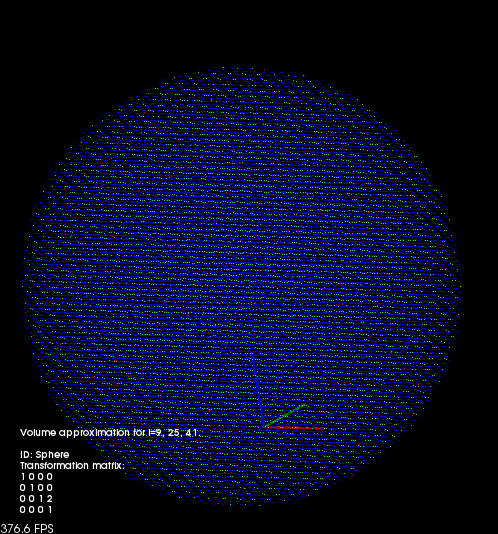
\includegraphics[width=2in]{./Results/sphere_vol}}&
    \adjustbox{valign=m}{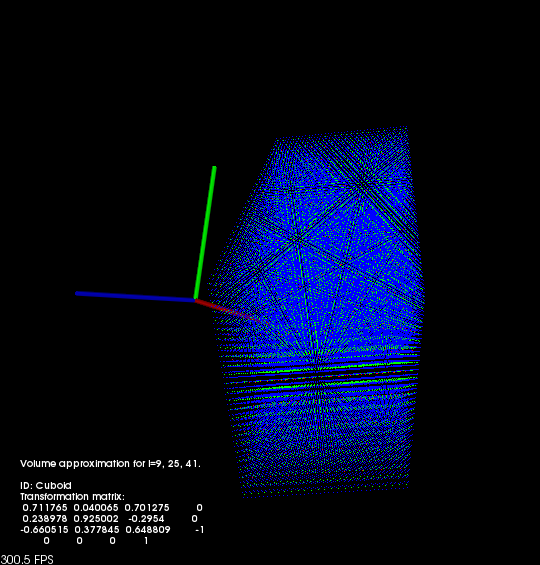
\includegraphics[width=2in]{./Results/cube_vol}}&
    \adjustbox{valign=m}{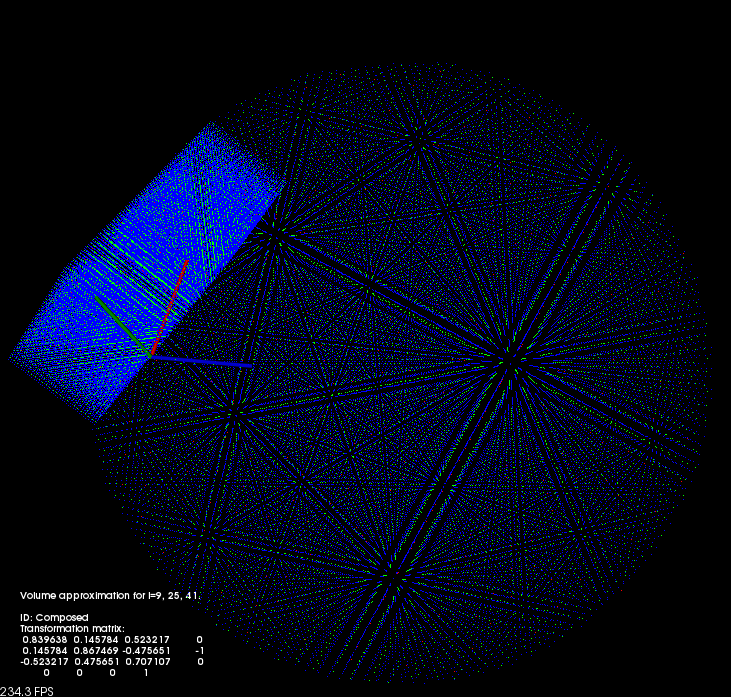
\includegraphics[width=2in]{./Results/compound_vol}} \\
    \adjustbox{valign=m}{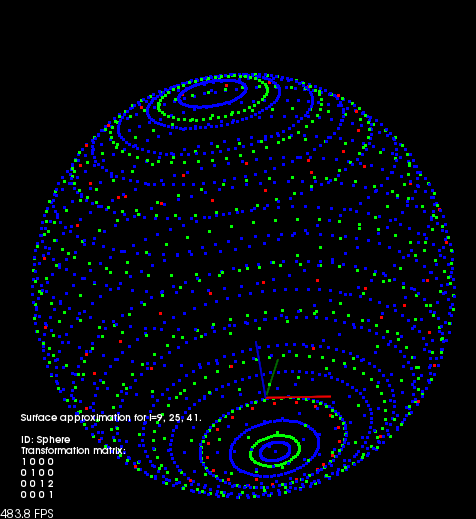
\includegraphics[width=2in]{./Results/sphere_surf}}&
    \adjustbox{valign=m}{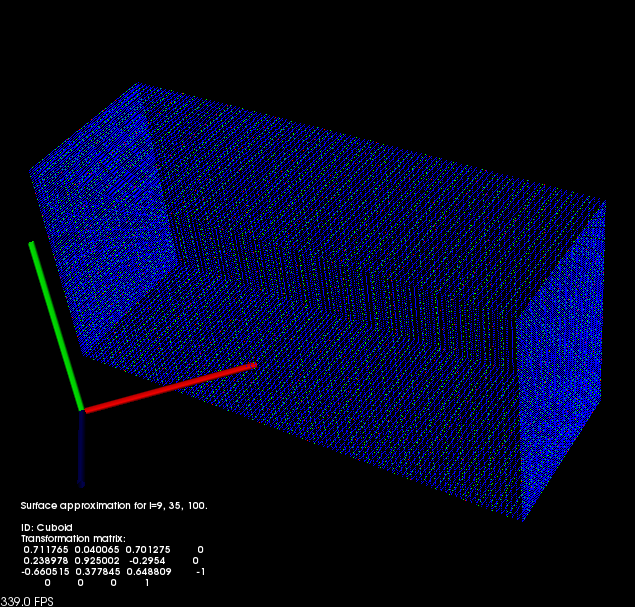
\includegraphics[width=2in]{./Results/cube_surf}}&
    \adjustbox{valign=m}{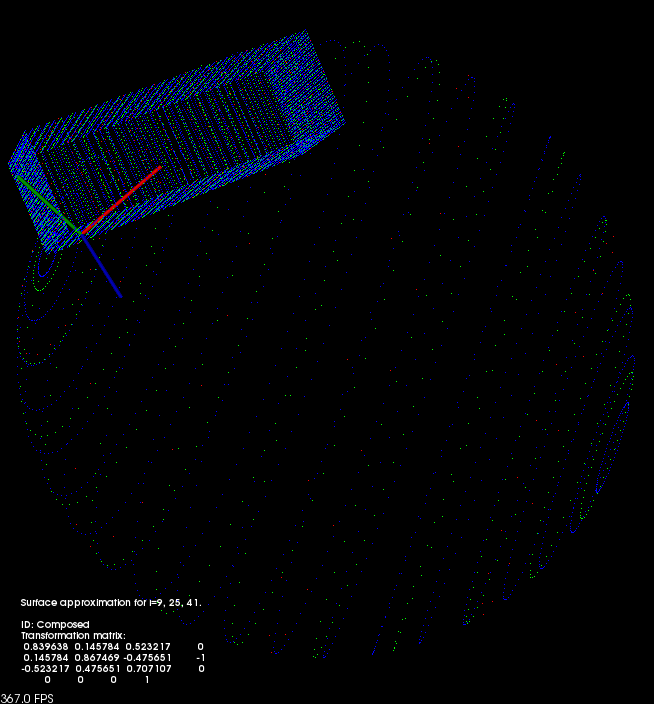
\includegraphics[width=2in]{./Results/compound_surf}}
  \end{tabular}
  \caption{Surface (top) and volume (bottom) approximation of a cube (left), a sphere (center) and a compound
  (right) for different values of $l$, depicted in red, green, and blue. \label{fig:approximate_shapes}}
\end{figure}

\subsection{Volume computation via central points} \label{volume-via-points}
After getting the approximation of the shape as a set of points, the
intersection volume is trivial to compute: as each shape knows how to check
whether a points is contained into it, it is sufficient to count the number of
points which it contain, and then assume that each point corresponds to the same
fraction of the shape's volume: $V_{\text{cube}}=\frac{V_{\text{shape}}}{N_p}$.
This assumption will be valid for sure, i.e. the computed sum will converge to
the actual intersection value if $l$ is high enough, thanks to the third
property of the approximation function stated in eqn.
\ref{eqn:points_with_constant_density}.

The total intersection volume $V_{\text{int}}$ computed with approximation level
$l$ will then be
\begin{equation}
  V_{\text{int}}(l)=V_{\text{shape}} \frac{N_{\text{in}}}{N_p(l)}
\end{equation}

\subsection{Optimized volume computations for particular cases}
The method presented in sec. \ref{volume-via-points} is universally valid,
being able to be applied for every combination of shapes. However, this is
clearly not efficient if applied to large datasets; also, the computational
complexity increases cubically with the level of approximation as stated in
eqn. \ref{volume-l-3}. Thus, when performing intersections for shapes for which
a closed form solution is known, this is preferred. In this project the case of
sphere-sphere intersection has been implemented as an example, but other cases
can be easily added due to the polimorphic structure of the algorithm.

The volume of the intersection of two spheres $S_1$ and $S_2$ can be reduced to three cases which only
depend on the distance $d$ between the centres of the spheres and their radii
$R$ and $r$, with $R\geq r$:

\begin{equation}
  V_{int}\left(S_1,S_2\right)=\left\{\begin{array}{lcr}
      0 & \mbox{if} & d\geq R+r, \\
      \frac{\pi \left(R+r-d\right) ^2 \left(
      d^2 + 2dr - 3r^2 + 2dR + 6rR-3R ^2 \right) }{12d}
      & \mbox{if} & R-r<d<R+r, \\
      \frac{4}{3}\pi r^3 & \mbox{if} & d \leq R-r.
  \end{array}\right.
\end{equation}

\subsection{Computation skipping via surface and edges intersections}
Another consideration can improve a lot the execution speed of the algorithm:
due to the real-life nature of the application scenario, the gripper will
actually seldom hit more than one object at a time. Thus, if the algorithm is
able to detect if two objects actually intersect \emph{before} computing their
volume, the resulting speedup will be important.

A sufficient and necessary condition for two shapes $S_1$ and $S_2$ to intersect is that, fixing
one of the two, at least one point of the surface $B$ of the other must be contained
into the first, or viceversa:

\begin{equation} \label{eqn:no-surface-in-volume}
  V_{\text{int}}\left(S_1,S_2\right)\neq 0 \Leftrightarrow \left(\exists P \in
    B\left(S_1\right) : P \in S_2\right) \vee \left(\exists P \in
    B\left(S_2\right) : P \in S_2\right) 
\end{equation}

When computing an intersection, the volume can thus be set to $V_{\text{int}}=0$
if no point of the surface of each shape is contained into another; as
approximating the surface of each shape results in $O(l^2)$ points, the
computation time taken by the algorithm if this strategy is applied will be
reduced by a factor $l$ if the shapes don't intersect (which is the most
probable case, given the above heuristic considerations), while the penalty for
computing the surface in case of failure of the strategy will be negligible with
respect to the volume computation's execution time.

On the other size, if of of the two shapes is fully contained into the other
one, the intersection's volume is equal to the volume of the contained shape.
A sufficient and necessary condition for a shape $S_1$ to be fully contained into
another shape $S_2$ is that all of the points of the surface $B$ of the first
are contained into the second, and none of the points of the surface of the
second are contained into the first:

\begin{equation} \label{eqn:surface-in-volume}
  S_1 \in S_2 \Leftrightarrow \left( P \in S_2 , \forall P \in B(S_1) \right)
  \wedge \left( \not \exists P \in B(S_2) : P \in S_1 \right).
\end{equation}

A lot of special cases exists for these situations too, that can improve the
execution speed (although this is asymptotically negligible, as the average
execution time will already be $O(l^3)$); for example, for cube-to-sphere
intersection, eqn. \ref{eqn:surface-in-volume} can be reduced to constant time by
noticing that it is sufficient for all the vertices $V$ of the cube to be
contained into the sphere in order for its whole surface to be contained too;
more in general, for polygonal, convex, meshes-like shapes, only the edges must
be checked to be contained one into the volume of the other. Also, if the shapes
are \emph{simply connected}, the second part of eqn. \ref{eqn:surface-in-volume}
can be omitted as it is implicitly true if the first part is. The number of
points to check is thus halved or reduced to a constant number in these cases --
which actually represent the majority of cases.

\subsection{Final volume intersection algorithm}
The full algorithm used to compute shapes' intersections is stated
now. This applied is succession all of the heuristic considerations
stated in previous sections.\footnote{Most of these operations are
  actually, as already introduced, performed automatically into the
  implementation by the C++
  language's objects mechanism through inheritance. The algorithm is
  reported here in a procedural manner for clarity.}

When two shapes $S_1$ and $S_2$ have to be intersected, given their poses $P_1$ and $P_2$:
\begin{enumerate}
  \item{If either $S_1$ or $S_2$ are compound shapes, they are
    subdivided into their composing primitives and the intersection
    volume is computed separately for each pair of primitives. This
    will call this algorithm recursively with new values for $S_1$ and
    $S_2$, and is thus implemented automatically; the total
    intersection volume is then found by summing up all the resulting volumes;}
  \item{First, $S_1$ is queried to know if it has some heuristics to
    skip the computation of the intersection with $S_2$ in case of no
    intersection. The same is queried to $S_2$ to skip the
    intersection with $S_1$. If one of those queries is true, the
    corresponding heuristic is called; this can be considered an
    operation with no cost, so it is alright to call both the
    heuristics even if the two shapes are of the same type; the
    advantage which comes with this is that in case of different
    object types, each heuristic consideration has to be written only
    once, thus avoiding code redundancy;}
  \item{If at least one of the heuristic algorithms of step 2
    succeded, the intersection volume is set to $0$ and this algorithm
    exits;}
  \item{If there is the possibility of and intersection, the surface
    representation of $S_2$ is obtained and it is checked to see
    whether at least one point is contained into $S_1$. This is done
    so that $S_2$ is always the smaller (in volume) of the two shapes,
    to have higher spatial precision in the approximation and to
    exploit the count of these points in the next step.
    In order to
    have a probability $p=1$ of the two objects not to intersect if
    no points of $S_1$ belong to $S_2$'s surface, it
    would be needed to approximate the latter with infinite level of
    precision; in practice, the opposite path is taken and, starting
    from a minimal level of approximation  $l=2$, the algorithm moves
    on if at least one intersecting point has been found. If it
    doesn't, it exponentially increases the value of $l$ multiplying
    it of a factor $k$, and repeats
    the calculus until $l$ is higher than a threshold
    $t_{(p\approx 1)}$ for which it is reasonable to say that the
    objects don't actually intersect. Using this approach, at each
    step the number of points will increase of about a factor $k^2$
    due to the properties of the surface approximation function; this
    means that although the previous steps, with a lower $l$, are
    discarded if no intersections are there, the wasted time will be
    negligible with respect to the upcomping one, and so they introduced virtually no penalty;}
  \item{If at least one point of the surface is found which intersects
    the other shape, the actual count of these points is checked. If
    this is equal to the total number of points of the surface,
    this means that the intersection volume is equal to $S_2$ volume
    and the algorithm exits;}
  \item{If at least one point was found, but this is not equal to the
    total count of the points, the volume approximation algorithm is used to compute the
    actual intersection volume. The two shapes' volumes are computed,
    and the volume approximation is obtained for the shape with the
    smaller volume. This, at the same approximation level, will lead
    to a smaller absolute value on intersections as the smaller object
    will lead to approximating cubes with smaller volumes.}
\end{enumerate}

As it can be seen, this algorithm proceeds by steps, and each step is
computationally one order of magnitude bigger than the previous
one. This means that, if heuristic is used for the wrong reason, the
drop in performance will be negligible, as the steps which will have
to be done will require much more time to execute that what has been
wasted before. Also, in this way, the algorithm can be easily
parallelized, which is an obvious pro for it, and flexibility is
obtained easily: if, for example, intersection with a torus is needed,
it is sufficient to implement the two functions which approximate its
surface and volume with points, and heuristic algorithms can be left
apart for when their implementation will be needed. The whole codebase
will need no modification to work with the new shape.

